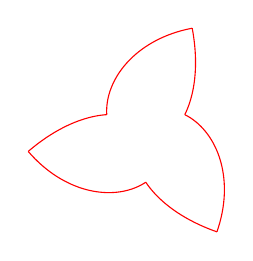
\begin{tikzpicture}[scale=0.7]

% Degrees to radians
\def\rad#1{(#1)/180*pi}

% Radians to degrees
\def\deg#1{(#1)*180/pi}

% r(θ)
\def \r#1#2{{(#1)*cos(#2)}, {(#1)*sin(#2)}}

\def \R{1.6}
\def \T{2.4}
\def \N{3}

\def \m{(\R/\T)}

% y0 in the paper
\def \y{(\R/(sqrt(\m*\m+1)*(exp((2 * pi * \m) / ((\m*\m+1) * \N)) - 1)))}

% θ1 in the paper
\def \theta {\deg{((1/\m) * ln(\R / (\y * sqrt(\m*\m+1)) + 1))}}

% θ2 in the paper
\def \phi {\deg{(\m * ln(\R / (\y * sqrt(\m*\m+1)) + 1))}}

% Increment in the angle of rotation of each petal
\def \dt{(360/\N)}

% Draw the N petals
\foreach \i in {1,...,\N}
{
  \draw [red, domain=-(90+\theta)+\dt*\i:-90+\dt*\i, samples=40] plot (\r{\y*exp(-\m*\rad{\x+90-\dt*\i})}{\x});
  \draw [red, domain=-90+\dt*\i:-(90-\phi)+\dt*\i, samples=40] plot (\r{\y*exp((1/\m)*\rad{\x+90-\dt*\i})}{\x});
}

% Draw the center
\tkzDefPoint(0, 0){O}
\tkzDrawPoint[color=red,fill=red](O)

\end{tikzpicture}
